% warwickthesis.tex modified by M Hadley from utthesis.doc  Sept 96
% Significant changes were made in 2009, first to work seemlessly with pdflatex
% and secondly to use the setspace package to control linespacing -
% removing some incompatibilities that existed before.
% any comments or problems - contact me  <m.j.hadley@warwick.ac.uk>
%%%%%%%%%%%%%%%%%%%%%%%%%%%%%%%%%%%%%%%%%%%%%%%%%%%%%%%%%%%%%%%%%%%%%%%%%%%%%
%%%
%%% File: utthesis.doc, version 2.0, January 1995
%%% =============================================
%%% Copyright (c) 1995 by Dinesh Das.  All rights reserved.
%%% This file is free and can be modified or distributed as long as
%%% you meet the following conditions:
%%%
%%% (1) This copyright notice is kept intact on all modified copies.
%%% (2) If you modify this file, you MUST NOT use the original file name.
%%%
%%% This file contains a template that can be used with the package
%%% utthesis.sty and LaTeX2e to produce a thesis that meets the requirements
%%% of the Graduate School of The University of Texas at Austin.
%%%
%%% All of the commands defined by utthesis.sty have default values (see
%%% the file
%           warwickthesis.sty
%%%                        for these values).  Thus, theoretically, you
%%% don't need to define values for any of them; you can run this file
%%% through LaTeX2e and produce an acceptable thesis, without any text.
%%% However, you probably want to set at least some of the macros (like
%%% \thesisauthor).  In that case, replace "..." with appropriate values,
%%% and uncomment the line (by removing the leading %'s).
%%%
%%%%%%%%%%%%%%%%%%%%%%%%%%%%%%%%%%%%%%%%%%%%%%%%%%%%%%%%%%%%%%%%%%%%%%%%%%%%%
% all comments starting with %! have been added by M Hadley as
% part of the conversion for the university of warwick
%
%
%\documentclass[11pt,a4paper,twoside]{report}      %% LaTeX2e document.
%%* Removed twoside option
\documentclass[11pt,a4paper]{report}      %% LaTeX2e document.
\usepackage[table]{xcolor}
\usepackage{warwickthesis,setspace,subfigure,graphicx}     %!  setspace is used to control linepacing
\usepackage[square]{natbib}                    %! needed for Harvard style of references.
% ! for more notes see the bibliography section below
\usepackage[nographicx]{incgraph}
\usepackage{algorithm}
\usepackage{algorithmicx}
\usepackage{algpseudocode}
\usepackage{amsmath, amsfonts}
\usepackage{enumerate}
\usepackage{amssymb}
\usepackage{geometry}
\renewcommand{\labelitemi}{\tiny$\blacksquare$}
\usepackage{algorithm,algorithmicx,algpseudocode}
\usepackage[toc,page]{appendix}


 % \usepackage[T1]{fontenc}
 % Choose one of the following (if not choosing the default,
%% viz., Computer Modern, font family):
% \usepackage{lmodern}
% \usepackage{mathpazo}
% \usepackage{kpfonts}
% \usepackage{mathptmx}
% \usepackage{times,mtpro2}
% \usepackage{txfonts}
% \usepackage{newtxtext,newtxmath}
% \usepackage{libertine}
% \usepackage[libertine]{newtxmath}
\usepackage[hang,bf]{caption}
\usepackage{hyperref}


\phdthesis                         %% use either, the default is \phdthesis.


%\thesisdraft                       %% Uncomment this if you want a draft
                                     %% version; this will print a timestamp
                                     %% on each page of your thesis.

 \rightchapter                      %% right-justified chapter headings.
                                     %% Chapter headings includes the
                                     %% Contents, Acknowledgments, Lists
                                     %% of Tables and Figures and the Vita.
                                     %% The default is \centerchapter.

\onehalfspacing                      %! This is the default and gives an acceptable "double spaced" thesis
                                     %! It is the minimum spacing accepted by the graduate school, and there is no reason to increase the spacing.
% \singlespacing                     %! Uncomment if you want single-spacing,
% \doublespacing                     %! uncomment if you want real double-spacing for some perverse reason.

%! Double sided printing is no longer allowed (March 2008), it caused too many problems at binding,
                              %\setlength{\evensidemargin}{0.15in}  %! Uncomment this line for double sided printing
                                      %! Double-sided printing has recently been
                                      %! allowed by the Graduate School (March 2003)
                                      %! The default is {0.7in} for single sided.
\newcommand{\bibfont}{\normalsize}

\DeclareMathOperator{\arcsinh}{arcsinh}
\renewcommand{\thesisdepartmentname}{Physics and Complexity Science}    %! The name of
                                                  %   the department

%! \renewcommand{\thesissubmission}{Submitted to the University of Warwick\\
%!              in partial fulfilment of the requirements\\
%!                   for admission to the degree of\\}
%!
%!!!!!!!! default is:
%!
\renewcommand{\thesissubmission}{Submitted to the University of Warwick\\
                        for the degree of}
%!
%! In the title page this wording will be preceeded by:  thesis\\
%!                 and ended by:  Doctor of Philosophy   (or the
%!                                               selected alternative names
%! use \\ where you want a new line

\renewcommand{\thesisauthor}{Anas A. Rana}    %% Your official name.

\renewcommand{\thesismonth}{January}     %% Your month of graduation.

\renewcommand{\thesisyear}{2014}      %% Your year of graduation.


\renewcommand{\thesistitle}{Stochastic Models for Cell Populations Undergoing Transitions}     %% The title of your thesis; use
                                     %% mixed-case.

%! \renewcommand{\thesistitletypesize}{\LARGE}   %! Put this in if you
                                  %!   want a Large title the default is \large

\renewcommand{\thesisauthorpreviousdegrees}{}
                                     %% Your previous degrees, abbreviated;
                                     %% separate multiple degrees by commas.

\renewcommand{\thesissupervisor}{Sach Mukherjee, Matthew Turner}
                                     %% Your thesis supervisor; use mixed-case
                                     %% and don't use any titles or degrees.

\renewcommand{\thesisauthoraddress}{}
                                     %% Your permanent address; use "\\" for
                                     %% linebreaks.
%! For the library declaration page only
%! \renewcommand{\thesiscopyrightagree}{agree}
                        %! agreement to allow single photocopies
%! \renewcommand{\thesiscopyrightagree}{do not agree}
                        %! refusal  to allow single photocopies
%! \renewcommand{\thesiscopyrightagree}{agree/do not agree}
                        %! undecided !!
                        %! default is agree


%%%%%%%%%%%%%%%%%%%%%%%%%%%%%%%%%%%%%%%%%%%%%%%%%%%%%%%%%%%%%%%%%%%%%%%%%%%%%
%%%
%%% The following commands are all optional, but useful if your requirements
%%% are different from the default values in utthesis.sty.  To use them,
%%% simply uncomment (remove the leading %) the line(s).

% \renewcommand{\thesisdegree}{...}  %% Uncomment this only if your thesis
                                     %% degree is NOT "DOCTOR OF PHILOSOPHY"
                                     %% for \phdthesis or "MASTER OF ARTS"
                                     %% for \mastersthesis.  Provide the
                                     %% correct FULL OFFICIAL name of
                                     %% the degree.

% \renewcommand{\thesisdegreeabbreviation}{...}
                                     %% Use this if you also use the above
                                     %% command; provide the OFFICIAL
                                     %% abbreviation of your thesis degree.

%\renewcommand{\thesistype}{Thesis}    %% Use this ONLY if your thesis type
                                     %! is NOT "Thesis"
                                     %% Provide the OFFICIAL type of the
                                     %% thesis; use mixed-case.

% \renewcommand{\thesistypist}{...}  %% Use this to specify the name of
                                     %% the thesis typist if it is anything
                                     %% other than "the author".

%%%
%%%%%%%%%%%%%%%%%%%%%%%%%%%%%%%%%%%%%%%%%%%%%%%%%%%%%%%%%%%%%%%%%%%%%%%%%%%%%


%\input header.tex          %! Input declarations, new
                              %theorems etc.


\begin{document}
% \setlength{\parindent}{0cm}

%%* Made default
% \thesiscopyrightpage                 %! Generate the copyright page.

%%* Uncomment a ttitle page.
 \thesistitlepage                     %% Generate the title page.
%\thesistitlecolourpage           %! Generates a COLOUR title page.

\newpage
\thispagestyle{empty}
\vfill
  \begin{figure*}
  \centering
  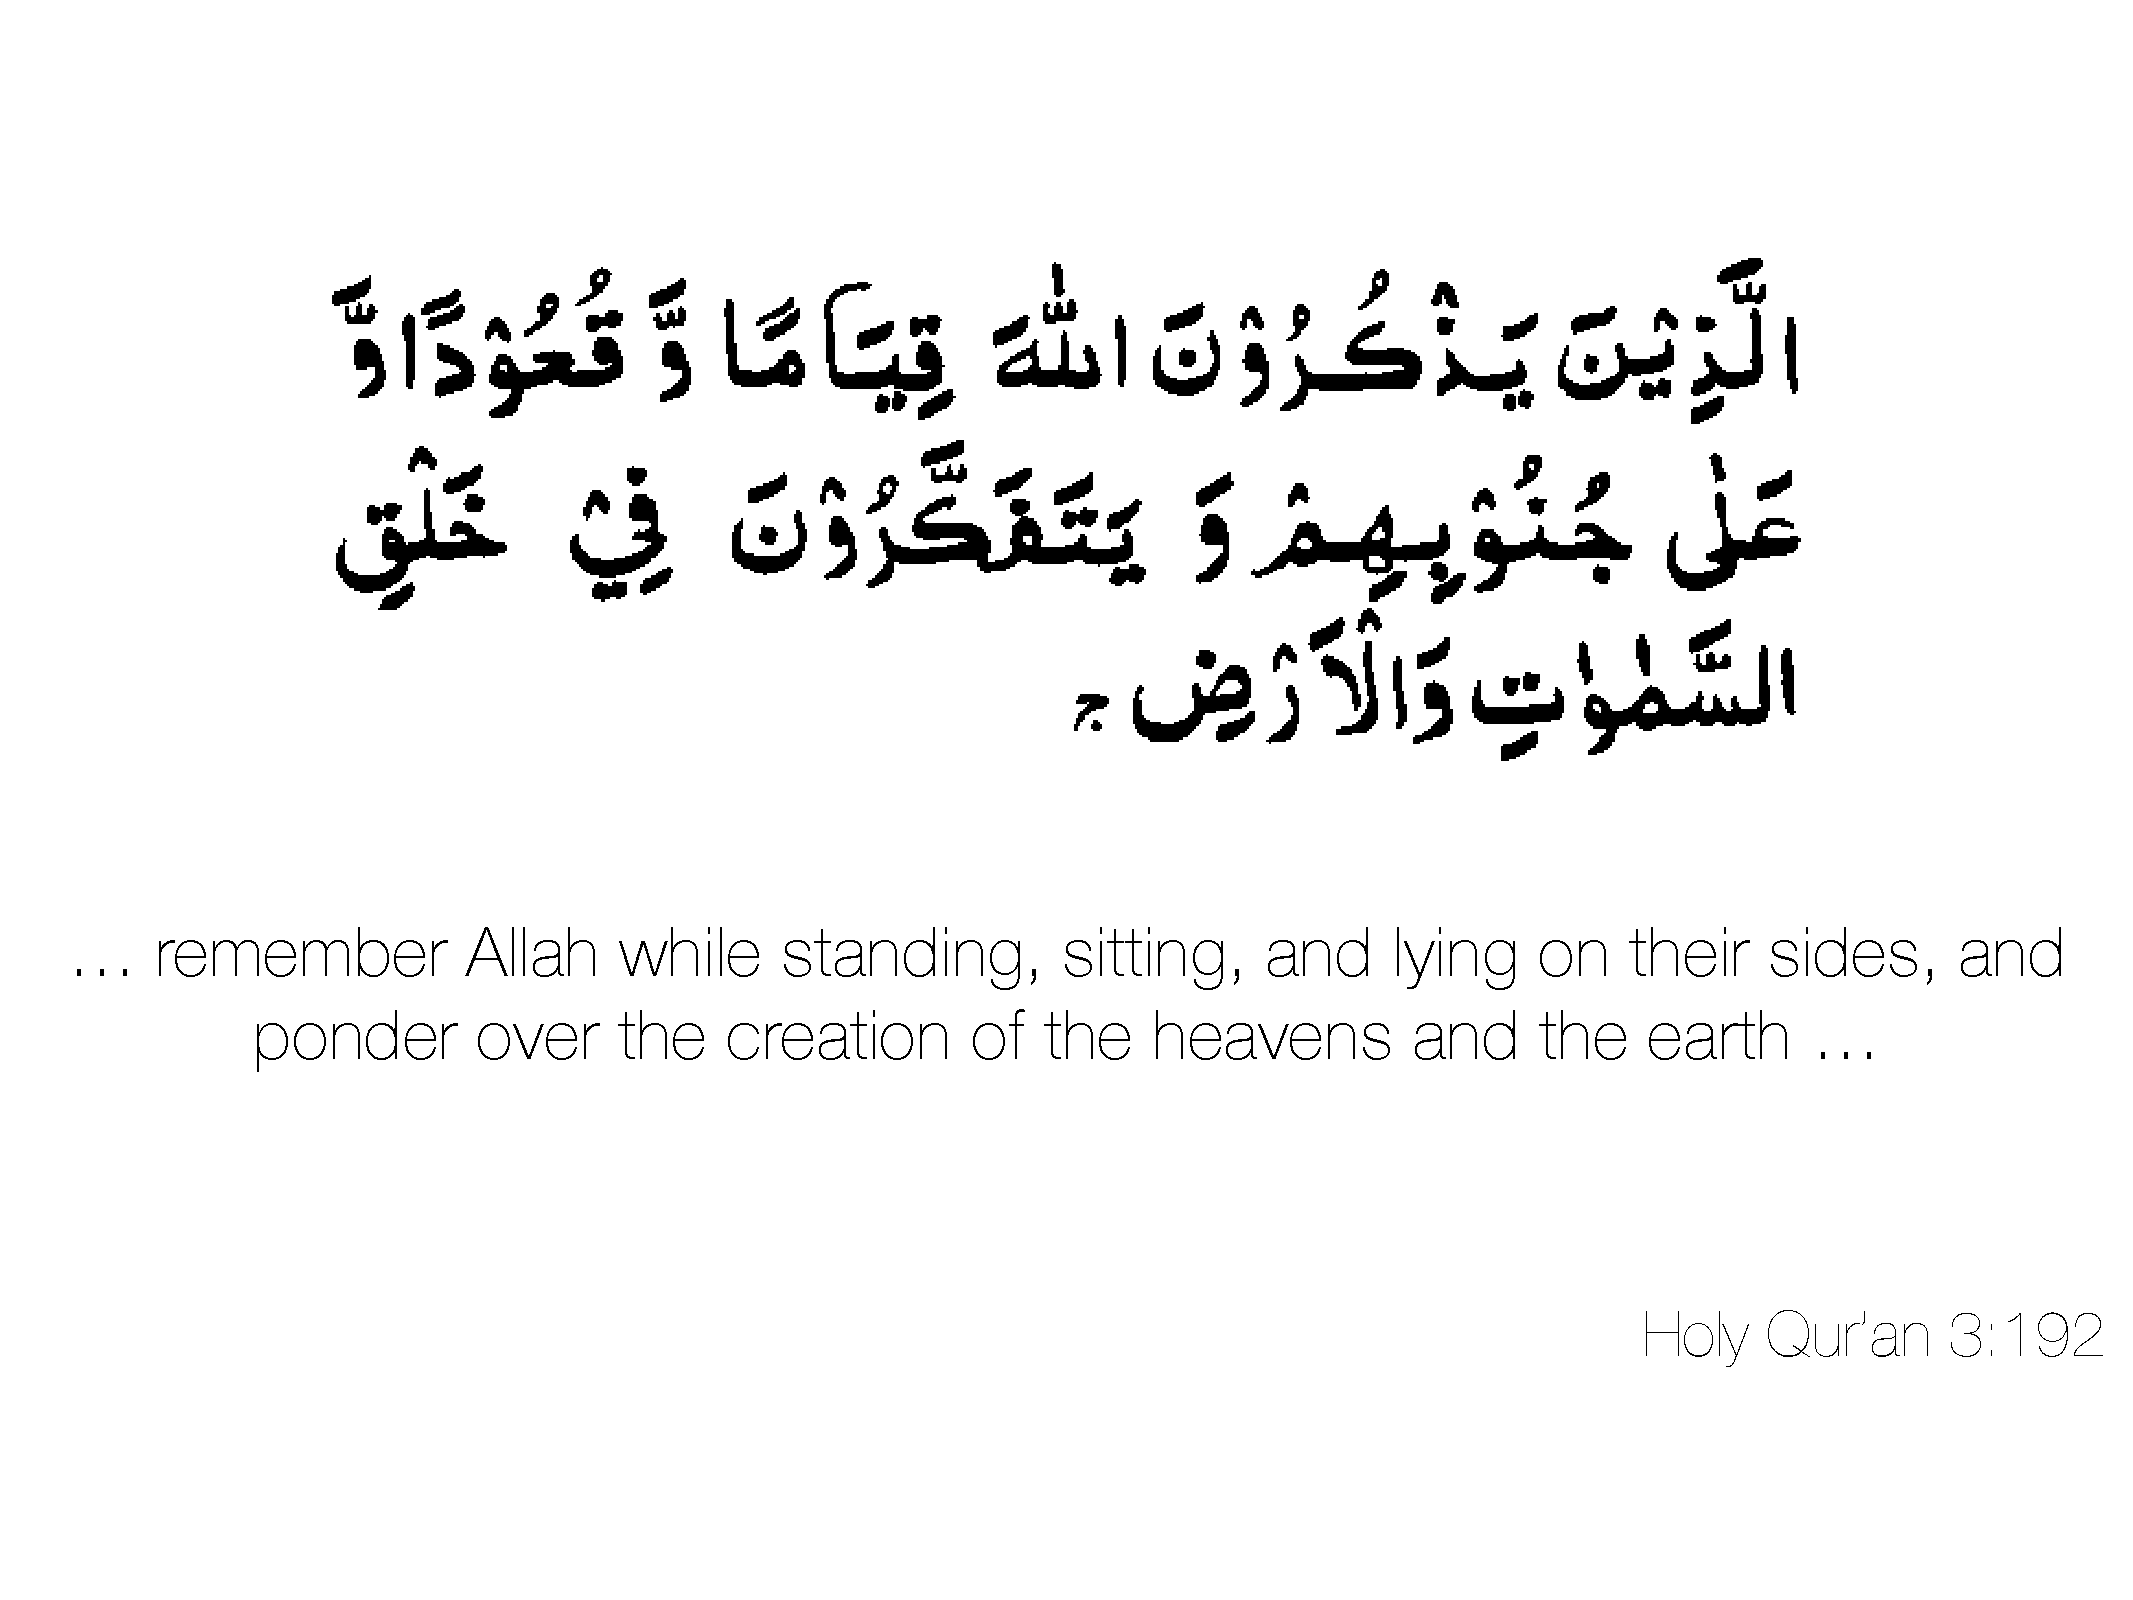
\includegraphics[width=1\textwidth]{pics/Verse.pdf}
  \end{figure*}
  \vfill

%%* Start roman page numbering here for contents, etc
\pagenumbering{roman} %! Begins roman numerals start from page i.

\tableofcontents                     %% Generate table of contents.
% \listoftables                      %% Uncomment this to generate list
                                     %% of tables.
% \listoffigures                     %% Uncomment this to generate list
                                     %% of figures.


\begin{thesisacknowledgments}        %% Use this to write your
\input ack.tex                    %% acknowledgments; it can be anything
                                     %% allowed in LaTeX2e par-mode.

\incgraph[paper=current]{pics/Acknowledgements_final.pdf}
\incgraph[paper=current]{pics/Acknowledgements_finalp2.pdf}


                                     %! This following is not needed, but you may like to add it.
%This \lowercase\expandafter{\thesistype} was typeset with
%\LaTeXe\footnote{\LaTeXe{} is an extension of \LaTeX. \LaTeX{} is
%a collection of macros for \TeX. \TeX{} is a trademark of the
%American Mathematical Society. The style package {\em warwickthesis} was
%used.} by \thesistypist.

\end{thesisacknowledgments}
\begin{thesisdeclaration}        %! Use this to declare the extent of

  The work contained here is my own except when otherwise stated. Any work based on collaborative efforts has been indicated including the extent of my contribution. The thesis has been written by myself and has not been submitted for any other degree at another university or institution.

  \begin{itemize}
  \item All experimental data analysed in this thesis was obtained by others and excluding Chapter \ref{cha:oncog-transf} is all separately published work.
  \item The work in Chapter \ref{cha:stamm} and the analysis of data in Chapter \ref{cha:oncog-transf} has been submitted for publication.
  \item The work in Chapter \ref{cha:stem-cells} has been published in \cite{Armond:2013} and my contributions to the work with some additional information are included here.
  \end{itemize}

\end{thesisdeclaration}


\begin{thesisabstract}               %% Use this to write your thesis
                                     %% abstract; it can be anything
                                     %% allowed in LaTeX2e par-mode.
 \begin{singlespace}       %! uncomment this if you need single spacing
   \input abstract.tex       %!           don't forget the end spacing!
                                     %! It must fit on one page.
                                     %! single spacing and smaller
                                     %! font size
                                     %!  is allowed here.
  \end{singlespace}
\end{thesisabstract}

%\begin{thesisabbreviations}       %! Use this to give a list of
                                   %! abbreviateons
                                   %! It can be anything
%\end{thesisabbreviations}         %! allowed in LaTeX2e par-mode.
                                   %!The following may be useful':
                     %!\begin{itemize}
                     %!     \item[symbol]descriptive text..
                     %!\end{itemize}

%\end{thesisabbreviations}

%\newpage{\pagestyle{empty}\cleardoublepage} %! ensure that Chapter 1 starts on an odd
                                           %! page when using double sided printing.
%%* Start arabic numbering of main text here
\pagenumbering{arabic} %! Begins arabic numerals start from page 1.

\input introduction.tex

\chapter{Background}
\input background.tex

\input background-math.tex

\input background-bio.tex

\chapter{State transitions using aggregated Markov models}
\label{cha:stamm}
\input stamm.tex

\chapter{Oncogenic transformation}
\label{cha:oncog-transf}
\input mcf10a.tex

\chapter{Stem cell reprogramming}
\label{cha:stem-cells}
 \input reprogramming.tex

\chapter{Cell cycle}
\label{cha:cell-cycle}

\input cell-cycle.tex


\input discussion.tex

%!!!!!!!!!!!!!!!

\begin{appendices}
  \input appendix-stamm.tex
  \input appendix-oncogenic.tex
\end{appendices}




% \bibliographystyle{plainnat}
\bibliographystyle{apa-good}
\bibliography{thesis-new}            %% Start your bibliography here;
                                 %! with sample.bib as your bibliography file. You can
                               %% also use:
                %! \begin{thebibliography}
                %!    \bibitem{etc....
                %! \end{thebibliography}
                               %% to generate your bibliography.

%\begin{thesisauthorvita}             %% Write your vita here; it can be
%                                     %% anything in LaTeX2e par-mode.
%\end{thesisauthorvita}               %%


\end{document}                       %% Done.
